% The price of verifiability in PIR, two-page version. Build with `make report` (latexmk, pdflatex), which writes
% docs/report.pdf. Every number below is a row of README.md's claims table, with the notebook cell that computes it.
\documentclass[10pt,a4paper,twocolumn]{article}
\usepackage[T1]{fontenc}
\usepackage{newtxtext,newtxmath}
\usepackage[margin=1.5cm,columnsep=0.6cm]{geometry}
\usepackage{graphicx}
\usepackage{booktabs}
\usepackage{enumitem}
\usepackage[font=footnotesize,labelfont=bf,skip=3pt]{caption}
\usepackage{microtype}
\usepackage[hidelinks]{hyperref}

\graphicspath{{figures/}}
\setlist{nosep,leftmargin=*,topsep=1pt}
\setlength{\parskip}{2pt}
\setlength{\parindent}{0pt}
\setlength{\textfloatsep}{6pt}
\setlength{\dbltextfloatsep}{6pt}
\setlength{\floatsep}{4pt}
\raggedbottom

\makeatletter
\renewcommand\section{\@startsection{section}{1}{\z@}{5pt plus 2pt minus 1pt}{1.5pt}{\normalfont\normalsize\bfseries}}
\makeatother

\newcommand{\x}{\ensuremath{\times}}
\newcommand{\cell}{128\,MiB\,\x\,1\,KiB}
\newcommand{\src}[2]{\emph{(notebook #1, cell #2)}}

\begin{document}
\twocolumn[{\centering
  {\Large\bfseries The price of verifiability in PIR: a common-hardware re-evaluation}\\[4pt]
  Iman Kalyan Chakraborty (2026801003) \quad Shambhavi Gantla (2026801014)\\[2pt]
  CS4406, 13 November 2026\\[2pt]
  {\small Code, raw results and notebooks: \url{https://github.com/astrion-coder/cs4406-sem-project}}\par\vspace{6pt}}]
\small

\section*{Summary}

Verifiable private information retrieval (PIR) lets a client fetch a record without revealing which one, and detect a
server that answers wrongly. Each paper reports its scheme's cost against its own baseline, on its own hardware. We
ran the authors' code for eight configurations on one Apple M1 Pro laptop, under one measurement harness, over
databases from 1\,MiB to 1\,GiB and records from 32\,B to 8\,KiB.
\begin{itemize}
  \item \textbf{The papers mostly reproduce.} 32 of 57 published targets pass outright, and 10 more differ only by
    our hardware being faster.
  \item \textbf{The cost falls in a different place for each scheme.} VeriSimplePIR (S1) costs nothing extra per
    query, but its offline phase takes about four times the baseline's server time. Colombo et al.'s Merkle scheme
    (M1) has almost no offline cost, but with 32\,B records each query costs up to 14\x{} the baseline's server time
    and 23\x{} its bytes.
  \item \textbf{Every check caught every fault we injected}, and no honest answer was rejected. Asking another replica
    after a rejection costs about two queries. Rebuilding VeriSimplePIR's state costs over 4,000.
  \item \textbf{Updates and the network change which scheme is cheaper. Load and cores do not.} Under concurrent
    load, each verifiable configuration's throughput overhead matches its single-query server-time overhead within
    5\,\%.
\end{itemize}
\texttt{README.md} lists every number here with the notebook cell that computes it. RQ1 to RQ7 and gate G7 are
defined in \texttt{vpir\_bench\_spec.md} (\S2 and \S12).

\section{Configurations and method}

Three configurations do not verify and are the baselines. \textbf{S0-go} is SimplePIR in the authors' Go code,
\textbf{S0-cpp} is the 64-bit SimplePIR inside the VeriSimplePIR code base, and \textbf{M0} is classic two-server XOR
PIR from Colombo et al.'s code. Five verify. \textbf{S1} and \textbf{S2} are VeriSimplePIR with and without its
honest-digest assumption. Upstream does not implement the one-time digest check the full scheme needs, so S2 runs
without it. \textbf{S3} and \textbf{S4} are Colombo et al.'s single-server authenticated PIR over integrity-amplified
LWE and over DDH, and both retrieve one bit per query. \textbf{M1} is Colombo et al.'s two-server Merkle-tree
authenticated PIR. We compare each verifiable configuration with the baseline from its own code base, S1 and S2
against S0-cpp and M1 against M0. The two-server schemes assume the servers do not collude, so a cost comparison
across families is not a security equivalence.

Every run uses one Apple M1 Pro with 6 performance and 2 efficiency cores and 16\,GiB RAM, on macOS with Go 1.27 and
Homebrew clang. The upstream code targets x86 Linux. We ported it with build-only patches, and ported
\texttt{dpf-go}'s x86 assembly to Go's AES library, checked bit for bit against the original under Rosetta. All three
upstream test suites pass natively. Each configuration has an adapter that calls the library the way its own tests
do, and no adapter uses the fake or random preprocessing that some upstream benchmarks default to.

The offline phase and the online phase each run in a fresh process, single-threaded, with at least 5 offline and 30
online repetitions (3 offline at 1\,GiB). A cell may use at most 14\,GiB, and we record a cell that needs more as out
of memory. Each run is on AC power and compares wall and monotonic time to catch sleep. We report medians. Overhead
is median(verifiable) / median(baseline), with a paired bootstrap 95\,\% interval over 10,000 resamples. The adapters
inject faults by changing the serialised server message, never the cryptographic code. The Tier 1 grid covers 4
database sizes by 4 record sizes for the six record-size configurations, S3 at four sizes and S4 at 64\,KiB to
1\,MiB. S4 takes 342\,s per digest at 1\,MiB, so we extrapolate its larger sizes from a linear fit.

\section{RQ1: do the papers' numbers hold?}

We checked 57 published targets against our runs. 32 pass outright. 10 differ by a hardware factor, because our
laptop is faster in absolute time than the papers' servers. S0-go reads 19.3\,GB/s on one core against SimplePIR's
10\,GB/s on a c5n.metal. 7 compare against a different baseline than the paper used, 7 are missing because the cell
does not fit in memory, and 1 needs explaining. The 16 byte counts we could measure are all within 20\,\% of the
papers', and 12 are within 3\,\%.

The overhead ratios mostly hold. M1 over M0 stays under the paper's 2.9\x{} bound for user time and 1.8\x{} bound for
bandwidth. S2 over S0-cpp is 1.33 to 1.49\x, inside VeriSimplePIR's reported 1.27 to 1.5\x. S3 costs 52\x{} SimplePIR
at 1\,MiB, inside Colombo et al.'s 30 to 100\x. The one miss is M1 over M0 at 1\,GiB, 1.55\x{} against the paper's
1.9\x. Our M0 query takes 0.20\,s against the paper's 0.13\,s, while M1 takes 0.32\,s against 0.25\,s, so the
baseline lost more to the hardware change than the verifiable scheme did.

\section{RQ2: what does verifiability add to one query?}

Figure~\ref{fig:f2} gives the overhead per online query over the whole grid.
\begin{itemize}
  \item \textbf{S1 costs nothing extra online.} Its server time is 0.98 to 1.02\x{} S0-cpp's, its client time at
    most 1.07\x, and it sends the same bytes. Its whole cost is in the offline phase, where the server proves the
    digest correct.
  \item \textbf{S2 costs up to 2.19\x} S0-cpp's server time and 1.50\x{} the bytes, both at 1\,MiB\,\x\,8\,KiB. The
    overhead falls as the database grows.
  \item \textbf{M1 is expensive with small records.} At 128\,MiB\,\x\,32\,B it takes 14.1\x{} M0's server time and
    sends 23.2\x{} the bytes, because each answer carries a Merkle proof that is large next to a 32\,B record. With
    8\,KiB records M1 costs 0.98 to 1.03\x{} M0's server time.
\end{itemize}

\begin{figure*}[t]
  \centering
  \begin{minipage}[b]{0.38\textwidth}
    \centering
    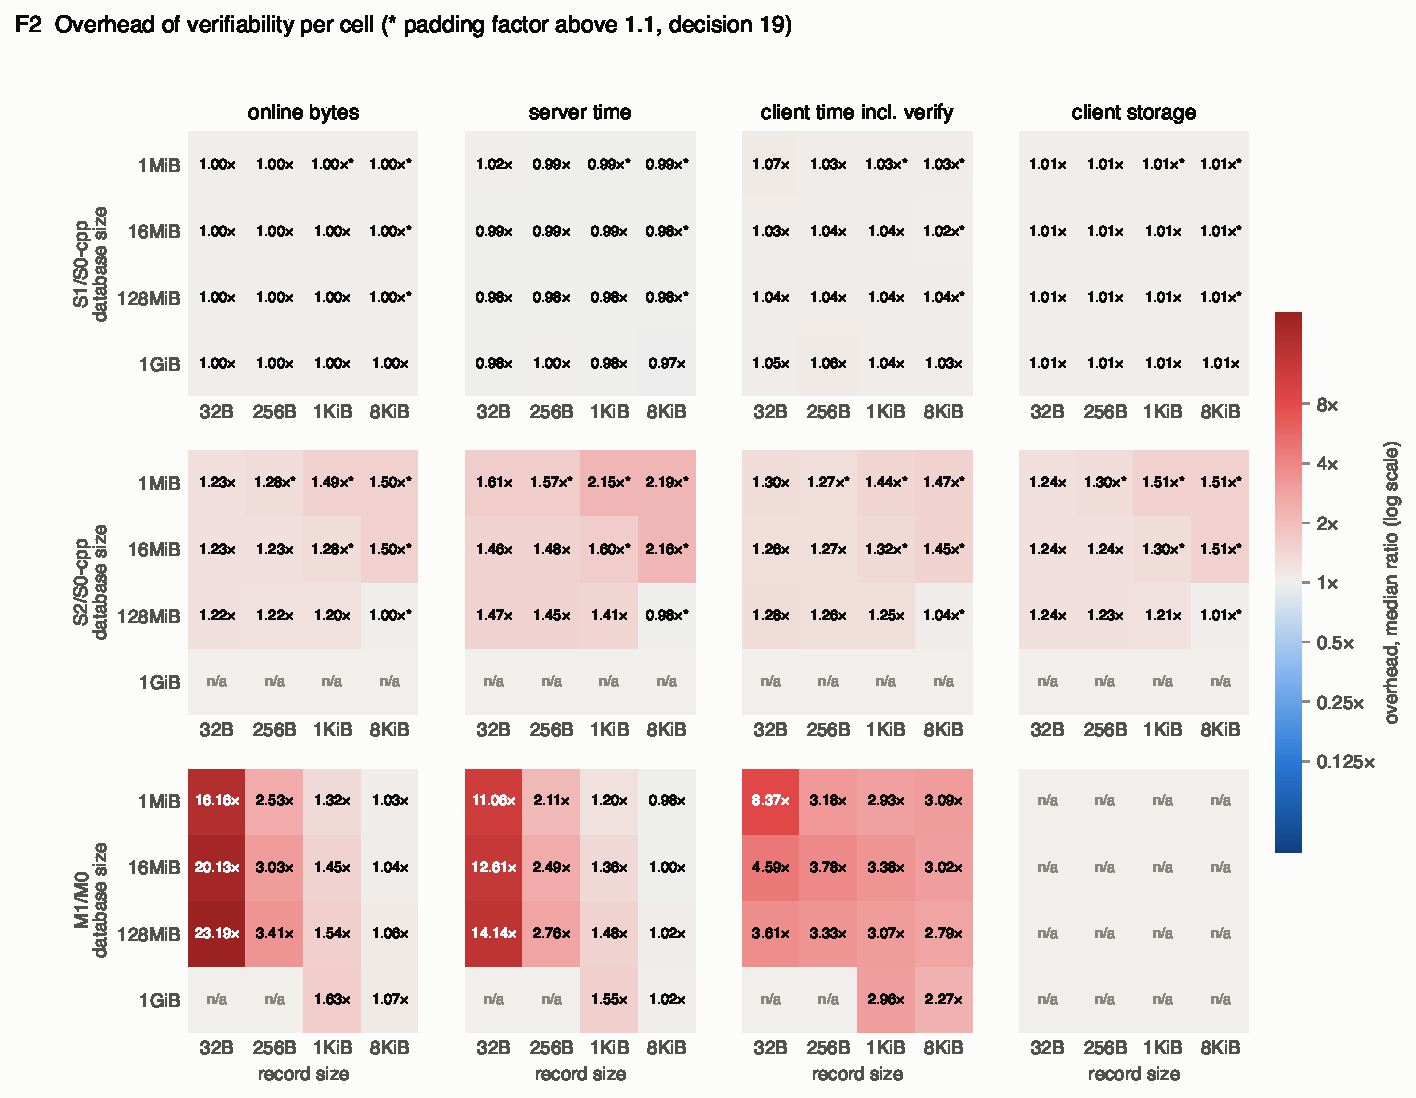
\includegraphics[width=\linewidth]{F2_overhead_heatmaps}
    \caption{Overhead of each verifiable configuration over its baseline across the grid \src{19}{4}.}
    \label{fig:f2}
  \end{minipage}\hfill
  \begin{minipage}[b]{0.6\textwidth}
    \centering
    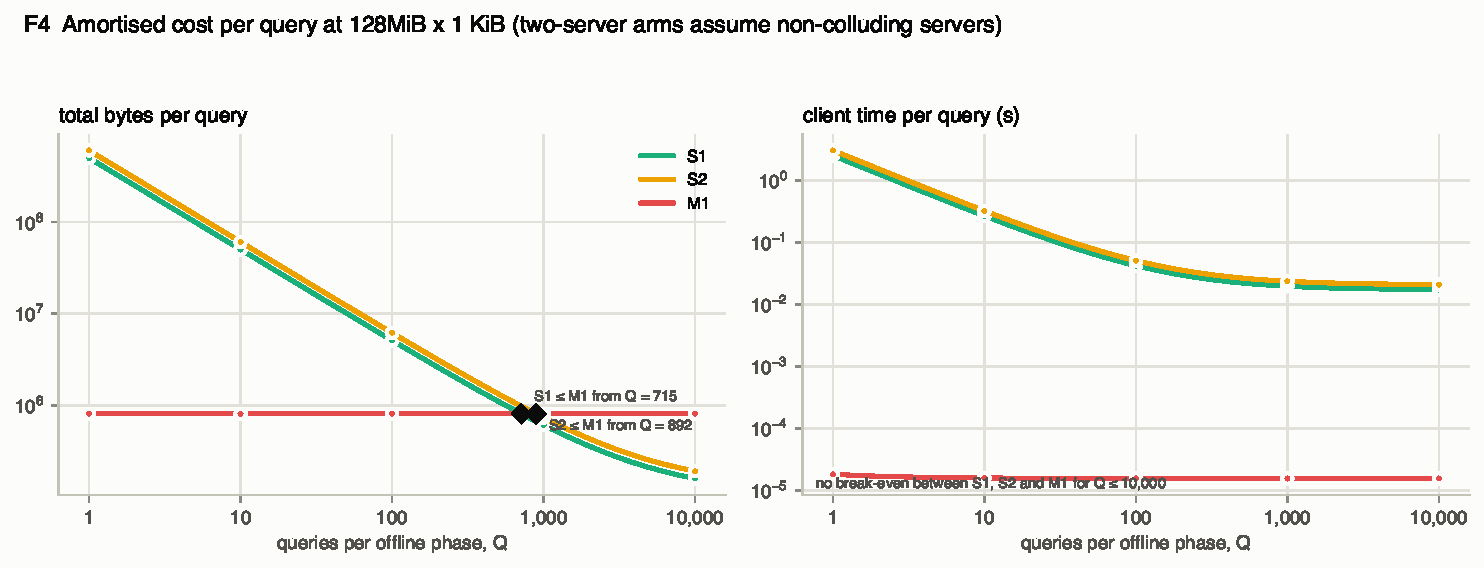
\includegraphics[width=\linewidth]{F4_amortised}
    \caption{Amortised cost per query against the number of queries $Q$ \src{21}{5}.}
    \label{fig:f4}
  \end{minipage}
\end{figure*}

\section{RQ3a: does the cost amortise over many queries?}

The single-server schemes pay before the first query. The client downloads a hint, 213\,MiB for S0-cpp and 476\,MiB
for S1 at \cell, and each query is then cheap. The two-server schemes pay per query. We priced a session of $Q$
queries as one offline phase plus $Q$ online queries, from the grid's medians (Figure~\ref{fig:f4}). In a direct run
of one cold offline phase and 100 queries in one process, every measured session total was within 2.4\,\% of the
computed one.
\begin{itemize}
  \item \textbf{Within a family, verification does not amortise in practice.} S1's offline phase takes about four
    times S0-cpp's server time. S1's server answers 2\,\% faster, so in server time S1 catches up only after 357,550
    queries at 128\,MiB. S2 and M1 never catch up with their baselines, because they cost more on every query.
  \item \textbf{Across families, the answer depends on which resource is scarce.} In bytes, S1 becomes cheaper than
    M1 after 715 queries at 128\,MiB and 454 at 1\,GiB. In client plus server time it takes 25,852 queries at
    128\,MiB and 7,075 at 1\,GiB.
  \item \textbf{S3 is costly per bit.} At 128\,MiB, retrieving one bit costs 2.0\,s and 3.4\,MB of traffic even at
    $Q = 10{,}000$.
\end{itemize}

\section{RQ3b: does the cost change over a real network?}

We ran 30 queries per configuration at \cell{} over loopback and over two links emulated with macOS dummynet,
broadband (100/20\,Mbit/s, 20\,ms round trip) and mobile (10/5\,Mbit/s, 60\,ms). We did not run the LAN profile,
because dummynet cannot emulate its 0.5\,ms round trip. A model that adds the grid's online compute time, the bytes
over the link's bandwidth and the measured round trips predicts the emulated latency. For the six record
configurations the emulated median is 1.002 to 1.084\x{} the model.

The network changes the overhead only where bytes differ. S1 sends exactly the bytes S0-cpp sends, and its latency
overhead stays at 1.01 to 1.03\x{} on every link. S2 sends 1.20\x{} the bytes. Its latency overhead is 1.34\x{} over
loopback, where compute dominates, and 1.22\x{} on broadband and mobile, where transfer dominates. M1 sends 1.54\x{}
M0's bytes, and its latency overhead is 1.37 to 1.46\x. On mobile a query takes 0.19 to 0.76\,s for the record
configurations, against 0.016 to 0.043\,s over loopback, so the link sets the user's wait and the verification does
not.

\section{RQ4: do the checks catch a cheating server?}

At \cell, the adapters corrupted the server's answer four ways, with a flipped bit, a wrong record, a stale record
and a withheld answer. Every verifiable configuration rejected every faulted answer, 200 of 200 for S1, S2 and M1
and 60 of 60 for S3 and S4. The baselines accepted every flipped, wrong and stale answer and noticed only the
withheld one. No honest answer was rejected in 3,385 to 5,817 sweep queries per configuration.

Detecting a fault costs little, but recovering from one can cost a lot. Aborting costs 0.82 to 1.00\x{} a fault-free
query, and asking another replica costs 1.82 to 2.00\x. Recomputing the preprocessed state, VeriSimplePIR's only
option when the digest itself is bad, costs 4,240\x{} a query for S1 and 4,655\x{} for S2.

\section{RQ5: what does an update to the database cost?}

None of the three code bases updates its state in place, so we assume each update forces a full rebuild and take its
cost from the grid's offline medians (Table~\ref{tab:rebuild}). M0 keeps no state. S1's rebuild is 3.9\x{} S0-cpp's
server time, while M1's Merkle tree rebuilds in under a second.

\begin{table}[h]
  \centering
  \footnotesize
  \begin{tabular}{lrrl}
    \toprule
    Configuration & Server (s) & Client (s) & Client downloads \\
    \midrule
    S0-cpp (baseline) & 33.5 & 0 & 213\,MiB hint \\
    S1 & 131.5 & 2.5 & 476\,MiB hint and proof \\
    S2 & 189.4 & 3.0 & 575\,MiB \\
    M1 & 0.78 & 0.00 & 32\,B root \\
    S3 (one bit) & 111.3 & 0.00 & 138\,MiB \\
    \bottomrule
  \end{tabular}
  \caption{One rebuild after an update at \cell{} \src{24}{2}.}
  \label{tab:rebuild}
\end{table}

With $u$ updates per query, a query costs its online time plus $u$ rebuilds. At one update per 100 queries, an S1
query costs 1.37\,s against 0.032\,s with no updates, and an M1 query costs 0.045\,s. Rebuilding takes half of S1's
cost at one update per 4,155 queries, against one per 21 queries for M1. At 1\,GiB an S1 rebuild takes 1,073\,s
of server time, so a database that changes more than a few times an hour cannot keep S1's verified state current on
this machine.

\section{RQ6 and RQ7: load and cores}

Each configuration served \cell{} from one process with $W$ worker threads, and a load generator on the same machine
replayed 64 recorded queries against it. Each load point ran 3 times, with a 5\,s warm-up and a 30\,s measured
window. The load generator's CPU use peaked at 17\,\%, under gate G7's 70\,\% limit, so it never limited the
measurement.

\textbf{Under load, the overhead is the single-query overhead.} At $W = 6$, S0-go saturated at 731 queries/s, S0-cpp
and S1 at 379, S2 at 257, M0 at 127 and M1 at 89. The baseline's saturation throughput over the verifiable one's is
1.000 for S1, 1.474 for S2 and 1.435 for M1, against single-query server-time ratios of 0.982, 1.415 and 1.478. At
90\,\% of saturation, S0-cpp and S1 answer within 0.055\,s at the 95th percentile, S2 within 0.086\,s, M0 within
0.19\,s and M1 within 0.25\,s.

\textbf{Across cores, the overhead holds.} The single-server configurations reach 3.92 to 4.04\x{} their
one-worker throughput at $W = 4$ (3.13\x{} for S3) and 4.83 to 5.69\x{} at $W = 6$. M0 and M1 reach 3.16 and 3.19\x{} at $W = 4$ and
gain nothing more at $W = 6$, because their two servers then run 12 workers on 8 cores. The overhead varies across
$W$ by at most 0.8\,\% for S1, 1.0\,\% for M1 and 3.0\,\% for S2.

\section{What we found in the upstream code}

\begin{itemize}
  \item \textbf{SimplePIR's query path mis-addresses packed entries.} When several entries share one
    $\mathbb{Z}_p$ element, upstream's \texttt{Query} and \texttt{Recover} still address the element, not the entry.
    With real setup on a one-bit database most queries panic or return a wrong bit. Our adapter addresses packed
    entries itself.
  \item \textbf{A corrupted Merkle proof makes M1's client try to allocate tens of GiB.}
    \texttt{merkle.DecodeProof} sizes an allocation from the proof's first four bytes before reading any hash, so a
    cheating server can exhaust the client's memory. The adapter refuses these decodes and records them as
    rejections.
  \item \textbf{VeriSimplePIR leaks memory per phase.} Its matrix type has no destructor. The adapter runs offline
    repetitions in a child process, and the leaked memory is freed when the child exits.
  \item \textbf{Colombo et al.'s current classic two-server PIR is not the paper's.} Since October 2024 its client
    sends DPF keys. We pinned the commit before that change, where it sends XOR shares as the paper describes.
\end{itemize}

\section{Limits}

\begin{itemize}
  \item \textbf{Ratios, not absolute times.} Our machine is an ARM laptop and the papers used x86 servers, so we
    compare overhead ratios with the papers.
  \item \textbf{Implementation, not only scheme.} A ratio across code bases mixes scheme cost with engineering, so
    every overhead pair stays within one code base.
  \item \textbf{Memory.} With 16\,GiB of RAM, S2 and S3 do not fit at 1\,GiB, and M1 at 1\,GiB fits only with
    records of 1\,KiB and up.
  \item \textbf{S2 is not the full scheme.} Upstream lacks the digest check, so S2's overhead understates the paper's
    full VeriSimplePIR.
  \item \textbf{Tier 2 runs at one cell.} RQ3a, RQ3b, RQ4, RQ6 and RQ7 run at \cell, so they say nothing about how
    their effects change with size.
  \item \textbf{No core pinning.} macOS cannot pin threads, so a single-threaded run may move between performance and
    efficiency cores.
\end{itemize}
The full list is in \texttt{docs/threats\_to\_validity.md}. \texttt{make all} reruns the Tier 1 grid,
\texttt{make session-check}, \texttt{make netem} and \texttt{make concurrency} rerun Tier 2, and \texttt{make report}
builds this PDF.

\end{document}
